\usepackage{listings}

\lstdefinestyle{CustomPython}{
  backgroundcolor=\color{codebg},
  basicstyle=\ttfamily\footnotesize\color{black},
  keywordstyle=\color{keyword}\bfseries,
  commentstyle=\color{comment}\itshape,
  stringstyle=\color{string},
  tabsize=2,
  showstringspaces=false,
  breaklines=true,
  breakatwhitespace=true,
  language=Python,
  numbers=none,
}

\lstdefinestyle{bashstyle}{
  backgroundcolor=\color{codebg},
  basicstyle=\ttfamily\footnotesize\color{black},
  commentstyle=\color{comment}\itshape,
  stringstyle=\color{string},
  showstringspaces=false,
  tabsize=2,
  breaklines=true,
  breakatwhitespace=true,
  language=bash,
  numbers=none
}

\NewDocumentCommand{\snakeicon}{O{1em}}{
  \raisebox{-0.2\height}{
\includegraphics[height=#1]{assets/python}}
}
\NewDocumentCommand{\terminalicon}{O{1em}}{
  \raisebox{-0.2\height}{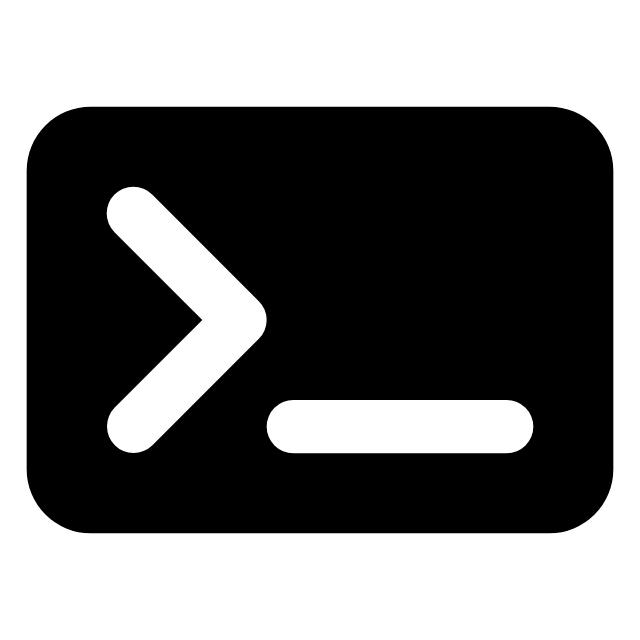
\includegraphics[height=#1]{assets/terminal}}
}

\newtcblisting{pythoncode}{
  listing only,
  listing options={style=CustomPython},
  colback=codebg,
  colframe=codeframe,
  coltitle=black,
  fonttitle=\footnotesize\ttfamily,
  title={\snakeicon\ Python},
  arc=2pt,
  boxrule=0.5pt,
  left=6pt,
  right=6pt,
  top=0pt,
  bottom=6pt,
  breakable,
  enhanced
}

\newtcblisting{bashcode}[1][]{
  listing only,
  listing options={style=bashstyle},
  colback=codebg,
  colframe=codeframe,
  coltitle=black,
  fonttitle=\footnotesize\ttfamily,
  title={\terminalicon\ Bash},
  arc=4pt,
  boxrule=0.5pt,
  left=6pt,
  right=6pt,
  top=0pt,
  bottom=6pt,
  enhanced,
  #1
}

\lstset{style=CustomPython}